%%%%%%%%%%%%%%%%%%%%%%%%%%%%%%%%%%%%%%%%%%%%%%%%%%%%%%%
% A template for Wiley article submissions.
% Developed by Overleaf. 
%
% Please note that whilst this template provides a 
% preview of the typeset manuscript for submission, it 
% will not necessarily be the final publication layout.
%
% Usage notes:
% The "blind" option will make anonymous all author, affiliation, correspondence and funding information.
% Use "num-refs" option for numerical citation and references style.
% Use "alpha-refs" option for author-year citation and references style.

\documentclass[alpha-refs]{wiley-article}
% \documentclass[blind,num-refs]{wiley-article}

% Add additional packages here if required
\usepackage{siunitx}

% Update article type if known
\papertype{Original Article}
% Include section in journal if known, otherwise delete
\paperfield{Journal Section}

\title{A Design for Phase II Clinical Trials in Stratified Medicine with Efficacy and Toxicity Outcomes and Predictive Variables}

% List abbreviations here, if any. Please note that it is preferred that abbreviations be defined at the first instance they appear in the text, rather than creating an abbreviations list.
\abbrevs{NSCLC, non-small-call lung cancer; PS2, performance status 2; PD-L1, programmed death-ligand 1.}

% Include full author names and degrees, when required by the journal.
% Use the \authfn to add symbols for additional footnotes and present addresses, if any. Usually start with 1 for notes about author contributions; then continuing with 2 etc if any author has a different present address.
\author[1]{Kristian Brock}
\author[1]{Christina Yap}
\author[1]{Laura Llewellyn}
\author[1]{Holly Smith}
\author[1]{Gillian McNab}
\author[2\authfn{2}]{Gary Middleton}
\author[1\authfn{2}]{Lucinda Billingham}
\contrib[\authfn{1}]{Professors Middleton and Billingham are joint senior authors of this work.}

% Include full affiliation details for all authors
\affil[1]{Cancer Research UK Clinical Trials Unit, University of Birmingham, Birmingham, B15 2TT, UK}
\affil[2]{Institute of Immunology and Immunotherapy, University of Birmingham, Birmingham, B15 2TT, UK}

\corraddress{Kristian Brock, Cancer Research UK Clinical Trials Unit, University of Birmingham, Birmingham, B15 2TT, UK}
\corremail{k.brock@bham.ac.uk}

%\presentadd[\authfn{2}]{Department, Institution, City, State or Province, Postal Code, Country}

\fundinginfo{Merck, Sharp \& Dohme}

% Include the name of the author that should appear in the running header
\runningauthor{Brock et al.}

% Custom operators
\DeclareMathOperator{\logit}{logit}

\begin{document}

\maketitle

\begin{abstract}
One of the primary goals of stratified medicine is to tailor the clinical trial decision to patient cohorts where there is evidence that outcomes are associated with predictive variables.
The design presented, BEBOP, incorporates predictive baseline information to jointly model efficacy and toxicity and selectively approve a treatment only in cohorts where it is shown to be acceptable, a posteriori.
We demonstrate in the context of PePS2, a phase II trial of pembrolizumab in performance status 2 non-small cell lung cancer patients.
Our predictive variables are PD-L1 expression level and pretreatment status. 
We show that model performance is good across a range of scenarios.
Key to this is that BEBOP shares information across cohorts. 
In contrast, beta-binomial models that operate on cohorts singly perform less well.
However, performance does not materially deteriorate when efficacy and toxicity are assumed independent, suggesting there is limited benefit to joint modeling in our scenario.
Nevertheless, BEBOP let us avoid the unappealing prospect of running parallel trials in cohorts in PePS2.


% Please include a maximum of seven keywords
\keywords{phase 2, efficacy, toxicity, stratified, personalised, predictive, baseline}
\end{abstract}



\section{Introduction}
\label{s:introduction}
There is a dearth of phase II clinical trial designs that incorporate predictive patient variables to assess efficacy and toxicity.
Our motivation is PePS2, a phase II trial of pembrolizumab in non-small-cell lung cancer patients.
We present BEBOP, a novel clinical trial design that uses predictive patient information to simultaneously study efficacy and toxicity.
In the rest of this section, we describe the trial setting and summarise existing, alternative clinical trial designs.
In Section \ref{s:alternative}, we present our proposed design.
In Section \ref{s:simulations}, we simulate performance for BEBOP in PePS2 and compare it to that of simple Bayesian beta-binomial conjugate models.
We discuss some limitations of our model and the potential for it to be used in other scenarios in Section \ref{s:discussion}.
Finally in Section \ref{s:conclusions} we finish with some conclusions.
In the supplementary appendix, we provide a detailed summary of alternative designs, advice on parameterising BEBOP, and explore alternative parameterisations.

\subsection{The PePS2 Trial}
\label{s:peps2}
PePS2 (EudraCT 2015-002241-55) is a phase II trial of pembrolizumab in non-small-cell lung cancer (NSCLC) patients with Eastern Cooperative Oncology Group (ECOG) performance status 2 (PS2).
A patient with PS2 is ambulatory and capable of self-care but typically too ill to work.
Critically, it is doubtful that a PS2 patient could tolerate the toxic side effects of chemotherapy.
This is particularly problematic because there are currently very few alternative therapies.

The primary objective of PePS2 is to research if pembrolizumab is associated with sufficient efficacy with acceptably low toxicity to justify use in performance status 2 patients.
The joint primary outcomes are (i) \textit{toxicity}, defined as the occurrence of a treatment-related dose delay or treatment discontinuation due to adverse event; 
and (ii) \textit{efficacy}, defined as stable disease (SD), partial response (PR) or complete response (CR) for at least 18 weeks, as measured by RECIST v1.1\citep{Eisenhauer2009}, also referred to as \textit{durable clinical benefit}.

Pembrolizumab inhibits the programmed cell death 1 (PD-1) receptor via the programmed death-ligand 1 (PD-L1) protein.
In a phase I study with 495 patients, \cite{Garon2015} showed pembrolizumab to be active and tolerable in performance status 0 \& 1 NSCLC patients.
Overall, 19.4\% of patients had an objective response (PR or CR) and 9.5\% experienced an adverse event of grade 3 or higher.
The rate of toxicity compares favourably to those typically seen in advanced NSCLC patients using chemotherapy \citep{Schiller2002, Borghaei2015}.
We foresee no reason why the rates of efficacy and toxicity should not be similar in PS2 patients, thus we hope to show that pembrolizumab is a viable treatment in this specific patient population.

Garon \textit{et al.} introduce the PD-L1 proportion score biomarker, defined as the percentage of neoplastic cells with staining for membranous PD-L1, hitherto referred to as \textit{PD-L1 score}.
In the nomenclature of \cite{Buyse2011}, they demonstrate PD-L1 to be a \textit{valid} and \textit{predictive} biomarker of pembrolizumab activity.
Efficacy outcomes for the 313 patients in their validation group, allocated to cohorts based on PD-L1 score, are shown in Table \ref{tab:garon.efficacy}.
Objective responses are observed in all cohorts and the probability of response generally increases with PD-L1 score.
They do not report any heterogeneity with respect to toxicity.

\begin{table}[p]
	\centering
	\caption{Objective response rates in PD-L1 score cohorts for the 313 patients in the validation sample of Garon \textit{et al.}\cite{Garon2015}.}
	\label{tab:garon.efficacy}
	\begin{tabular}{|c | c | c |}
		\hline
		PD-L1 Cohort & Criteria & Objective Response \%, (95\% CI) \\ 
		\hline
		Low & PD-L1 score $<$ 1\% & 10.7 (2.3, 28.2) \\ 
		Medium & 1\% $\geq$ PD-L1 score $<$ 50\% & 16.5 (9.9, 25.1) \\ 
		High & PD-L1 score $\geq$ 50\% & 45.2 (33.5, 57.3)\\
		\hline
	\end{tabular}
\end{table}

Based on this information, we expect PD-L1 score to be predictive of response in our PS2 population.
Additionally, we expect a mix of patients that have and have not previously received treatment for their cancer.
In the Garon trial, 24.8\% of previously untreated patients achieved a response compared to 18.0\% of previously treated patients.
This represents a potentially small but important effect that should be considered when testing the treatment.
PD-L1 and pre-treatment status are our putatively predictive baseline variables in PePS2.

Given the dearth of alternative therapies, even a relatively low response rate would be attractive in PS2 patients.
Using the three Garon PD-L1 cohorts and two groups for pre-treatment status, each patient in PePS2 will belong to exactly one of six cohorts.
A design that formally stratifies accrual with recruitment targets in each cohort would ultimately exclude eligible patients before the trial has completed.
Instead, our preference is for an all-comers designs that admits all eligible patients, thus not stratifying in accrual, but uses the baseline information to stratify in the analysis, ultimately yielding a decision on the treatment in each cohort.
This naturally suggests analysis by regression model.

Pembrolizumab has not been investigated in PS2 patients so the clinical scenario requires a trial design that tests efficacy and toxicity.
Furthermore, the toxicity outcome pertains to events that hinder or cease drug administration.
In these circumstances, it is natural to conclude that the presence of a toxicity event in any particular patient would decrease the likelihood of an efficacy event.
Thus, the perfect design would study correlated co-primary outcomes.

Being a phase II trial, there is strong motivation to deliver findings quickly to inform potential phase III research in a timely manner.
It is felt that recruitment in the region of 60 patients over twelve months would be feasible but that recruitment materially higher could be difficult. 
The feasible trial size is modest because we are only admitting PS2 patients.
In the next section, we summarise the results of our search for a suitable clinical trial design.

PePS2 is a investigator-initiated and investigator-led trial funded by Merck, Sharp \& Dohme.

\subsection{Search for Feasible Trial Designs}
We searched the published literature for a trial design that admits explanatory data to study co-primary binary efficacy and toxicity outcomes, preferably allowing them to be associated. 
We summarise our findings here.
Full details are given in the supplementary information.

Trial designs for dose-finding using joint primary outcomes of efficacy and toxicity have been devised, including some extensions of the \cite{OQuigley1990} Continual Reassessment Method (CRM) \citep{Braun2002,Zhang2006, Mandrekar2010} and others using Bayesian adaptive designs \citep{Thall2004, Cook2006, Thall2014, Wages2014}.
Generally in such dose-finding models, dose (or transformed dose) is used as the sole explanatory variable that determines the outcome probabilities and therefore such approaches could be adapted to a non-dose-finding setting to incorporate other types of explanatory variables as required for PePS2. 

Designs that incorporate both efficacy and toxicity for the phase II setting have also been proposed. 
These include two-stage designs \citep{Jin2007, Brutti2011} and general group sequential designs \citep{Cook1994, Conaway1995, Conaway1996}.
Their emphasis is to develop stopping rules rather than incorporate predictive information.

In addition we studied review articles of biomarker-guided clinical trial designs \citep{Freidlin2010, Buyse2011, Antoniou2016} but none explicitly incorporate co-primary outcomes and were therefore not directly relevant to our situation. 

Probably the best-known and most widely used design for a single arm phase II trial with co-primary outcomes of efficacy and toxicity is that proposed by \cite{Bryant1995}. 
Using a Bryant \& Day optimal design to contrast efficacy rates of 10\% and 30\% and toxicity rates of 10\% and 30\%, with efficacy and toxicity significance of 10\% and overall power of 80\%, requires the final analysis to use 27 patients.
If we were to use this design in each PePS2 cohort, we would require $6 \times 27 = 162$ patients, an infeasibly high number.
Even if we were to ignore the potentially important information in the pre-treatment variable and analyse three PD-L1 cohorts, we would still require 81 patients using parallel Bryant \& Day designs.
Furthermore, the design assumes that the patient population is homogeneous.
Using it to test any combination of our cohorts would involve ignoring baseline data that we strongly suspect to be informative. 
We declined to do this.
Our preference was for a model-based design that could increase power by incorporating validated predictive information.

With no published design available that would be suitable for PePS2, we devised a new design adapted from the dose-finding model proposed by \cite{Thall2004}. 
The aim of this paper is to introduce the design and demonstrate its use in the PePS2 trial. 




\section{Methods}
\label{s:alternative}
In this section, we describe a novel Bayesian trial design that models the probabilities of efficacy and toxicity using  predictive variables. 
We call the design BEBOP, for Bayesian Evaluation of Bivariate Outcomes with Predictive variables.
BEBOP allows a treatment acceptance/rejection decision for each permutation of the predictive variables, facilitating the consideration of patient cohorts.
First we describe a probability model for associated bivariate binary outcomes, borrowed from Thall \& Cook\cite{Thall2004}.


\subsection{Bivariate Binary Probability Model}
We redeploy the probability model at the core of the \textit{EffTox} design for dose-finding by \cite{Thall2004} .
The authors use logit models, $\pi_E(x, \boldsymbol{\theta})$ and $\pi_T(x, \boldsymbol{\theta})$, for the marginal probabilities of efficacy and toxicity, where $x$ is the transformed dose-level and $\boldsymbol{\theta}$ is a vector of parameters.
They define variables $a$ and $b$ that take the value 1 if a patient experienced efficacy and toxicity respectively, else 0, and allow the outcome probabilities to associate using the \textit{Gumbel} model presented in \cite{Murtaugh1990}.
The joint probability of efficacy and toxicity events $a, b$ at dose $x$ is:
\begin{gather}
\label{eqn:prob.model}
\pi_{a,b} = \pi_E^a (1-\pi_E)^{1-a} \pi_T^b (1-\pi_T)^{1-b}+ (-1)^{a+b} \pi_E (1-\pi_E) \pi_T (1-\pi_T) \frac{e^\psi - 1}{e^\psi + 1}
\end{gather}
where the $(x, \boldsymbol{\theta})$ notation has been suppressed for brevity.
Here, $\psi$ models the association between efficacy and toxicity events.
As $\psi \to -\infty$, the fraction at the end of (\ref{eqn:prob.model}) tends to -1.
Similarly, as $\psi \to \infty$, the fraction tends to 1.
In this regard, the fraction can be interpreted as the correlation between efficacy and toxicity, determined by the value of $\psi \in \mathbb{R}$.

Priors must be specified for each element of $\boldsymbol{\theta}$.
The authors provide practical advice on how to do this\cite{Thall2004, Thall2014}.

\subsection{BEBOP}
\label{sec:bebop}
We reuse in BEBOP the probability model of Thall \& Cook described above with predictive patient variables in place of dose-level.
Generally, for patients with predictive variable vector $x$, the marginal probabilities of efficacy and toxicity are modeled using the logit models:
\begin{equation}
\label{eqn:bebop.efficacy}
\logit \pi_E(x, \boldsymbol{\theta}) = g(x, \boldsymbol{\theta})
\end{equation}
and 
\begin{equation}
\label{eqn:bebop.toxicity}
\logit \pi_T(x, \boldsymbol{\theta}) = h(x, \boldsymbol{\theta})
\end{equation}
where $\boldsymbol{\theta}$ is the vector of all parameters in the model.
The exact specifications of $g$ and $h$ are left for the trialists to specify.
Generally, as with all statistical models, $g$ and $h$ should be both plausible and parsimonious.
We present our choices for the PePS2 trial in the next section.

For trial data
\begin{equation}
\boldsymbol{X} = \{(x_1, a_1, b_1), ..., (x_n, a_n, b_n) \}
\end{equation} 
the aggregate likelihood function is
\begin{equation}
\mathcal{L}(\boldsymbol{X}, \boldsymbol{\theta}) = \prod_{i=1}^n \pi_{a_i, b_i} (x_i, \boldsymbol{\theta})
\end{equation}
Let $\boldsymbol{\theta}$ have prior distribution function $f(\boldsymbol{\theta})$.
For patients with predictive variable vector $x_i$, the posterior expectation of the probability of efficacy under the treatment is 
\begin{equation}
\label{eqn:post.eff}
\mathbb{E}(\pi_E(x_i, \boldsymbol{\theta}) | \boldsymbol{X}) = \frac{\int \pi_E(x_i, \boldsymbol{\theta}) f(\boldsymbol{\theta})  \mathcal{L}(\boldsymbol{X}, \boldsymbol{\theta}) d\boldsymbol{\theta}}{\int f(\boldsymbol{\theta})  \mathcal{L}(\boldsymbol{X}, \boldsymbol{\theta}) d\boldsymbol{\theta}}
\end{equation}
and the posterior probability that the probability of efficacy exceeds $\pi_E^*$ is 
\begin{equation}
\label{eqn:post.acc.eff}
\Pr(\pi_E(x_i, \boldsymbol{\theta}) > \pi_E^*| \boldsymbol{X}) = \frac{\int \mathbb{I}(\pi_E(x_i, \boldsymbol{\theta}) > \pi_E^*) f(\boldsymbol{\theta})  \mathcal{L}(\boldsymbol{X}, \boldsymbol{\theta}) d\boldsymbol{\theta}}{\int f(\boldsymbol{\theta})  \mathcal{L}(\boldsymbol{X}, \boldsymbol{\theta}) d\boldsymbol{\theta}}
\end{equation}
where $\mathbb{I}(A)$ is the indicator function, taking value $1$ when $A$ is true, else 0.
Similar expressions can be derived for posterior estimates of the probability of toxicity and the probability that the probability of toxicity is less than some threshold $\pi_T^*$.

Further taking the lead from Thall \& Cook, we propose the treatment be approved in patients with predictive variable vector $x_i$ when it is sufficiently likely that the associated efficacy probability exceeds some minimum threshold, $\pi_E^*$, and toxicity probability is less than some maximum threshold, $\pi_T^*$.
The acceptance criteria are:
\begin{equation}
\label{eqn:acceptance}
\begin{split}
\Pr(\pi_E(x_i, \theta) > \pi_E^* | \boldsymbol{X}) > p_E \\
\Pr(\pi_T(x_i, \theta) < \pi_T^* | \boldsymbol{X}) > p_T
\end{split}
\end{equation}
where $p_E$ and $p_T$ are determined using clinician input and simulation.
Naturally, $\pi_E^*$, $\pi_T^*$, $p_E$ and $p_T$ can vary by patient cohort.
We could, for example, set the efficacy hurdle lower in pre-treated patients if a dearth of feasible alternative treatments dictates that a lower efficacy hurdle is nevertheless clinically relevant.

\subsection{BEBOP in PePS2}
\label{sec:bebop.peps2}
Let patient $i$ have vector of predictive values $x_i = (x_{1i}, x_{2i}, x_{3i})$ as listed in Table \ref{tab:cohorts}.

\begin{table}[p]
	\centering
	\begin{tabular}{|c|c|c|c|}
		\hline Cohort & Treatment status & PD-L1 category & $x_i$ \\ 
		\hline 
		1 & Treatment naive & Low & (0,1,0) \\ 
		2 & Treatment naive & Medium & (0,0,1) \\ 
		3 & Treatment naive & High & (0,0,0) \\ 
		4 & Pre-treated & Low & (1,1,0) \\ 
		5 & Pre-treated & Medium & (1,0,1) \\ 
		6 & Pre-treated & High & (1,0,0) \\ 
		\hline 
	\end{tabular} 
	\caption{Cohorts used in the BEBOP model in the PePS2 trial. $x_i$ shows the predictive variable vector for patients in that cohort.}
	\label{tab:cohorts}
\end{table}

Using these variables, we propose that the marginal probabilities of efficacy and toxicity be described by logit-models so that, for a patient with predictive data $x_i$:
\begin{align}
\label{eqn:logit}
\begin{split}
\logit \pi_E(x_i, \boldsymbol{\theta}) & = \alpha + \beta x_{1i} + \gamma x_{2i} + \zeta x_{3i} \\
\logit \pi_T(x_i, \boldsymbol{\theta}) & = \lambda
\end{split}
\end{align}
and associate $\pi_E$ and $\pi_T$ using the Gumbel model (\ref{eqn:prob.model}).
Including $\psi$, our parameter vector $\boldsymbol{\theta} = (\alpha, \beta, \gamma, \zeta, \lambda, \psi)$ has six elements.

Under the described model, the expected probability of efficacy is different for each distinct arrangement of $x_i$.
Furthermore, the log-odds of efficacy for treatment naive patients in the three PD-L1 categories are assumed to be a common linear shift of those for pre-treated patients in the same PD-L1 cohorts.
Figure \ref{fig:garon.response.logodds} shows the log-odds of objective response by PD-L1 cohort for pre-treated and treatment-naive patients in the validation cohort of the Garon study. 
The model we propose effectively assumes that the equivalent lines in our study using our definition of efficacy will be piecewise parallel.
We see that this assumption is supported in the High and Medium cohorts of the Garon study, but modestly violated in the Low cohort.
A more complicated alternative specification could remove the parallelism assumption by incorporating interaction terms for PD-L1 cohort and pre-treatment status.
This alternative model would require two extra parameters to handle interactions between $x_{1i}$ and $x_{2i}$, and $x_{1i}$ and $x_{3i}$, respectively.
We return to this in Section \ref{s:simulations}.

\begin{figure}[p]
	\centering
	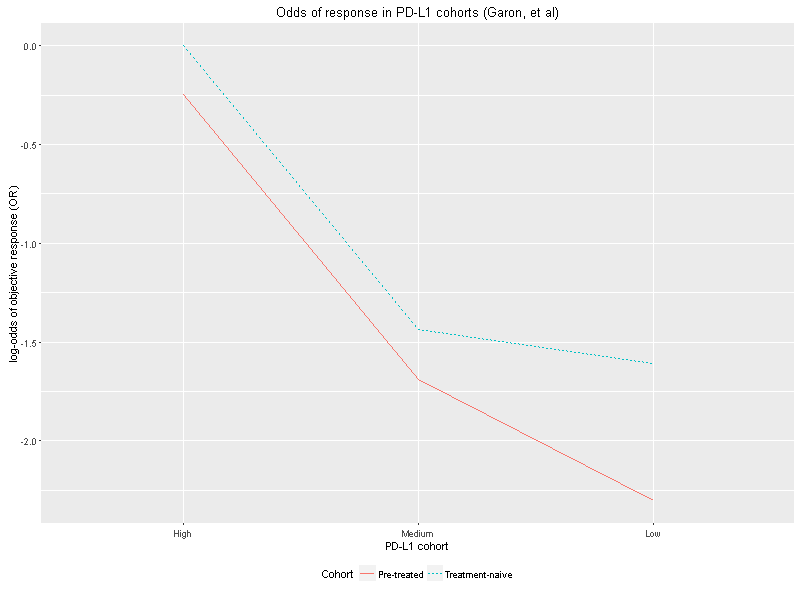
\includegraphics[width=\linewidth]{LogOddsOfResponseByCohort-Garon}
	\caption{Log-odds of objective response in PD-L1 cohorts in the validation sample (n=204) of the Garon \textit{et al.} study.}
	\label{fig:garon.response.logodds}
\end{figure}

In contrast, the probability of toxicity is assumed constant across all cohorts.
\cite{Garon2015} do not report in the main paper or supplementary appendix any difference in toxicity in the different PD-L1 or pre-treatment groups.
More-recently, \cite{Herbst2016} also did not report heterogeneity in pembrolizumab toxicity in NSCLC patients.

We must specify priors for the elements of $\boldsymbol{\theta}$.
We choose very modestly informative priors so that the prior mean probabilities of efficacy and toxicity are approximately 20\% in all cohorts, broadly reflecting our expectations.
Our efficacy and toxicity outcome definitions differ to used by \cite{Garon2015} and our patient population is similar but ultimately distinct.
We seek variance hyperparameters that are informative enough to locate approximately 95\% of the prior belief on the efficacy and toxicity event rates in the practically feasible range of 0-90\%, yet weak enough to be ably dominated by data.
Our priors in Table \ref{tab:priors} yield the prior beliefs on the rates for efficacy and toxicity in each cohort shown in Table \ref{tab:paper_priors}.

\begin{table}[p]
	\centering
	\caption{Normal prior distributions for the elements of $\boldsymbol{\theta}$.}
	\label{tab:priors}
	\begin{tabular}{ | c | c | c | }
		\hline
		& $\mu$ & $\sigma^2$ \\
		\hline 
		$\alpha$ & -2.2 & 4 \\ 
		$\beta$ & -0.5 & 4 \\ 
		$\gamma$ & -0.5 & 4 \\ 
		$\zeta$ & -0.5 & 4 \\
		$\lambda$ & -2.2 & 4 \\ 
		$\psi$ & 0 & 1 \\ 
		\hline 
	\end{tabular} 
\end{table}

\begin{table}[ht]
\centering
\begin{tabular}{rrrrrrr}
 Cohort & ProbEffL & ProbEff & ProbEffU & ProbToxL & ProbTox & ProbToxU \\ 
 \hline
 1 & 0.00 & 0.21 & 0.95 & 0.00 & 0.21 & 0.86 \\ 
2 & 0.00 & 0.20 & 0.95 & 0.00 & 0.21 & 0.86 \\ 
  3 & 0.00 & 0.20 & 0.85 & 0.00 & 0.21 & 0.86 \\ 
  4 & 0.00 & 0.21 & 0.97 & 0.00 & 0.21 & 0.86 \\ 
  5 & 0.00 & 0.20 & 0.97 & 0.00 & 0.21 & 0.86 \\ 
  6 & 0.00 & 0.21 & 0.94 & 0.00 & 0.21 & 0.86 \\ 
  \end{tabular}
\caption{BEBOP prior mean probabilities of efficacy (ProbEff) and toxicity (ProbTox) with lower (L) and upper (U) limits of 95\% credible intervals.} 
\label{tab:paper_priors}
\end{table}

Our priors contain no information on whether there is an expected benefit to having a higher PD-L1 score or being treatment naive. 
The aim of this trial is to research these factors in the PS2 population thus we omit our expectations from the \textit{primary} analysis.
However, in alternative analyses in the supplementary information, we show the effect of using: i) informative priors, that expect higher efficacy in increasing PD-L1 cohorts, and in previously untreated patients; and ii) completely uninformative priors.

We choose $\pi_E^* = 0.1$ and $\pi_T^* = 0.3$ for all cohorts because these represent the thresholds beyond which the treatment would be considered not active enough or too toxic.
We sought values of $p_E$ and $p_T$ that would approve the treatment with approximately 90\% probability in a benchmark favourable setting (scenario 1 in Table \ref{tab:ocs}) and reject with at least 95\% probability in an adverse setting (scenario 2).
Using trial-and-error on small batches of simulations we arrived at $p_E = 0.7$ and $p_T = 0.9$.




\section{Simulation Study}
\label{s:simulations}
We conduct simulation studies to assess the operating characteristics of our BEBOP implementation.
The parameters chosen will affect performance so they should be driven by the clinical scenario, wherever possible.
Sample size will naturally play a large part in determining performance.
Increasing the number of patients is the typical method for providing more information to a clinical trial design.
At the very minimum, we are interested in estimating the probability that a design will correctly approve a treatment in a favourable scenario (analogous to power in a frequentist analysis) and incorrectly approve a treatment in an adverse scenario (analogous to statistical significance).
We expect both of these probabilities to improve with sample size.
Building on this minimum, we will be interested to estimate the performance of a design over a wider range of scenarios that reflect what we might encounter in the trial.

\subsection{Simulating cohort membership and outcomes}
Patients will belong to one of six cohorts.
The cohorts are enumerated 1,..,6 in Table \ref{tab:cohorts}.
For brevity and clarity when discussing the parameterisation of PePS2, we present cohort parameter values in that order.
For example, a true efficacy vector $(0.1, 0.2, 0.3, 0.4, 0.5, 0.6)$ depicts an efficacy probability of 0.2 in cohort 2.

We randomly sample cohort prevalences and patient-cohort memberships to allow variability from this source of uncertainty.
For iteration $j$, we sample cohort membership probabilities $\rho_j \sim Dirichlet(\hat{\rho})$, where $\hat{\rho} = (15.7, 21.8, 12.4, 20.7, 18.0, 11.4)$, for $j=1,...,J$ simulated iterations.
Patient-level allocations to cohorts $1,...,6$ were randomly sampled from multinomial distributions with probability vector $\rho_j$.
These choices are justified in the supplementary appendix.
Furthermore, equal cohort sizes are assessed by simulation and presented in the supplement.

A simulation scenario requires the specification of true efficacy and toxicity probabilities in each cohort, and the level of association between efficacy and toxicity events.
In each scenario, we simulated $J=10,000$ iterations.
In each iteration, we randomly sampled $N=60$ patients belonging to the six PePS2 cohorts using the method described.
We then randomly sampled binary efficacy and toxicity events with probabilities driven by the cohort memberships.
We simulated correlated efficacy and toxicity events mirroring the method used in the R package \texttt{binarySimCLF} \citep{binarySimCLF}, itself based on the work of \cite{Qaqish2003}.
The level of association is measured by odds-ratio. 
At the null value 1.0, efficacy is no more or less likely in the presence of toxicity.
With values less than 1, the events are negatively associated, i.e. the presence of one event makes the other event less likely.
This concurs with what we might expect in PePS2 for the reasons given above.


\subsection{Assessing operating characteristics by simulation}
\begin{table}[ht]
\centering
\begin{tabular}{rrrrrrrrrr}
  \hline
Scenario & Cohort & ProbEff & ProbTox & Odd & N & Eff & Tox & BEBOP & BetaBin \\ 
  \hline
1 & 1 & 0.300 & 0.1 & 1.0 & 9.4 & 2.8 & 0.9 & 0.896 & 0.572 \\ 
   & 2 & 0.300 & 0.1 & 1.0 & 13.1 & 3.9 & 1.3 & 0.915 & 0.684 \\ 
   & 3 & 0.300 & 0.1 & 1.0 & 7.5 & 2.2 & 0.7 & 0.904 & 0.503 \\ 
   & 4 & 0.300 & 0.1 & 1.0 & 12.4 & 3.7 & 1.2 & 0.908 & 0.660 \\ 
   & 5 & 0.300 & 0.1 & 1.0 & 10.8 & 3.2 & 1.1 & 0.901 & 0.603 \\ 
   & 6 & 0.300 & 0.1 & 1.0 & 6.9 & 2.1 & 0.7 & 0.878 & 0.489 \\ 
   \hline
2 & 1 & 0.100 & 0.3 & 1.0 & 9.4 & 1.0 & 2.8 & 0.026 & 0.045 \\ 
   & 2 & 0.100 & 0.3 & 1.0 & 13.1 & 1.3 & 3.9 & 0.026 & 0.038 \\ 
   & 3 & 0.100 & 0.3 & 1.0 & 7.5 & 0.7 & 2.2 & 0.025 & 0.044 \\ 
   & 4 & 0.100 & 0.3 & 1.0 & 12.4 & 1.2 & 3.7 & 0.021 & 0.040 \\ 
   & 5 & 0.100 & 0.3 & 1.0 & 10.8 & 1.1 & 3.3 & 0.022 & 0.040 \\ 
   & 6 & 0.100 & 0.3 & 1.0 & 6.9 & 0.7 & 2.1 & 0.025 & 0.047 \\ 
   \hline
3 & 1 & 0.300 & 0.1 & 0.2 & 9.4 & 2.8 & 0.9 & 0.897 & 0.587 \\ 
   & 2 & 0.300 & 0.1 & 0.2 & 13.1 & 3.9 & 1.3 & 0.916 & 0.695 \\ 
   & 3 & 0.300 & 0.1 & 0.2 & 7.5 & 2.2 & 0.7 & 0.905 & 0.519 \\ 
   & 4 & 0.300 & 0.1 & 0.2 & 12.4 & 3.7 & 1.3 & 0.907 & 0.670 \\ 
   & 5 & 0.300 & 0.1 & 0.2 & 10.8 & 3.2 & 1.1 & 0.901 & 0.611 \\ 
   & 6 & 0.300 & 0.1 & 0.2 & 6.9 & 2.1 & 0.7 & 0.879 & 0.498 \\ 
   \hline
4 & 1 & 0.167 & 0.1 & 1.0 & 9.4 & 1.6 & 0.9 & 0.460 & 0.348 \\ 
   & 2 & 0.192 & 0.1 & 1.0 & 13.1 & 2.5 & 1.3 & 0.685 & 0.488 \\ 
   & 3 & 0.500 & 0.1 & 1.0 & 7.5 & 3.7 & 0.8 & 0.982 & 0.630 \\ 
   & 4 & 0.091 & 0.1 & 1.0 & 12.4 & 1.1 & 1.3 & 0.282 & 0.165 \\ 
   & 5 & 0.156 & 0.1 & 1.0 & 10.8 & 1.6 & 1.1 & 0.483 & 0.338 \\ 
   & 6 & 0.439 & 0.1 & 1.0 & 6.9 & 3.0 & 0.7 & 0.920 & 0.590 \\ 
   \hline
5 & 1 & 0.167 & 0.3 & 1.0 & 9.4 & 1.6 & 2.8 & 0.061 & 0.080 \\ 
   & 2 & 0.192 & 0.3 & 1.0 & 13.1 & 2.5 & 3.9 & 0.090 & 0.092 \\ 
   & 3 & 0.500 & 0.3 & 1.0 & 7.5 & 3.7 & 2.2 & 0.130 & 0.163 \\ 
   & 4 & 0.091 & 0.3 & 1.0 & 12.4 & 1.1 & 3.8 & 0.041 & 0.034 \\ 
   & 5 & 0.156 & 0.3 & 1.0 & 10.8 & 1.6 & 3.3 & 0.063 & 0.067 \\ 
   & 6 & 0.439 & 0.3 & 1.0 & 6.9 & 3.0 & 2.1 & 0.121 & 0.167 \\ 
   \hline
6 & 1 & 0.167 & 0.1 & 0.2 & 9.4 & 1.6 & 0.9 & 0.458 & 0.362 \\ 
   & 2 & 0.192 & 0.1 & 0.2 & 13.1 & 2.5 & 1.3 & 0.684 & 0.500 \\ 
   & 3 & 0.500 & 0.1 & 0.2 & 7.5 & 3.7 & 0.7 & 0.982 & 0.644 \\ 
   & 4 & 0.091 & 0.1 & 0.2 & 12.4 & 1.1 & 1.3 & 0.281 & 0.175 \\ 
   & 5 & 0.156 & 0.1 & 0.2 & 10.8 & 1.6 & 1.1 & 0.483 & 0.347 \\ 
   & 6 & 0.439 & 0.1 & 0.2 & 6.9 & 3.0 & 0.7 & 0.918 & 0.589 \\ 
   \hline
\end{tabular}
\caption{Simulated operating characteristics. 
ProbEff and ProbTox are the true probabilities of efficacy and toxicity.
Odds denotes the ratio of odds of efficacy in patients that experience toxicity to those that do not.
Odds=1 corresponds to no association; values less than one convey that efficacy is less likely when toxicity is observed; and vice-versa.
N is the mean number of patients in a cohort; Eff and Tox the mean number of events.
BEBOP is the probability that treatment is approved by the BEBOP model; 
BetaBin the probability it is approved by a beta-binomial model.
10,000 iterations were used in each scenario.} 
\label{tab:ocs}
\end{table}

Table \ref{tab:ocs} shows performance in six simulated scenarios.
The scenarios chosen broadly reflect our expectations, driven by the Garon study, and the range of scenarios over which the design should perform well.
The simulated mean number of patients, and efficacy and toxicity events, are presented for each cohort.
The probability of approving the treatment via the BEBOP model is shown.
To give measure to the benefit of information sharing in BEBOP, we also present the probabilities of approval under cohort-specific beta-binomial Bayesian conjugate models.
With prior $\pi \sim Beta(\alpha, \beta)$, the posterior beliefs are $\pi | r, n \sim Beta(\alpha + r, \beta + n - r)$ where $n$ is the number of patients in a cohort and $r$ is the number of events observed.
Inferences are made on the posterior distribution.
A modestly informative $Beta(0.4, 1.6)$ prior on the rates of efficacy and toxicity was chosen to expect event rates of 20\%.
This provides a prior 95\% credible interval of (0.0\%, 80.5\%) on each event rate, narrower (thus slightly more informative) than the equivalent under the family of normal priors used in BEBOP in Table \ref{tab:paper_priors}.
As with BEBOP, we consider alternative priors for the beta-binomial models in the supplement.
Re-implementing the same decision criteria, the beta-binomial models should approve the treatment in a given cohort if $Pr(\pi_E > 0.1 | r_E, n) > 0.7$ and $Pr(\pi_T < 0.3 | r_T, n) > 0.9$.

In scenarios 1 and 2, the rates of efficacy and toxicity are uniform across the cohorts.
Scenario 1 shows that if the true probability of efficacy is 30\% and toxicity is 10\%, we can expect BEBOP to approve the treatment with at least 87\% probability in all cohorts. 
The cohorts have different approval probabilities because the average cohort sizes are different. 
For example, cohort 6 has the smallest expected size and marginally lower approval probabilities.
A key benefit of the BEBOP design is the apportioning and sharing of information across cohorts via the Bayesian regression model.
For instance, BEBOP will quite reliably approve the treatment in scenario 1 in cohorts 3 and 6, even though they each only receive approximately 7 patients who experience 2 efficacies.
The high efficacy rate observed in other cohorts informs BEBOP.

Despite having a slightly more informative prior, the beta-binomial model would approve the treatment approximately 50\% of the time in scenario 1, as shown in the BetaBin column of Table \ref{tab:ocs}.
With seven patients, the median size of this cohort, the beta-binomial model must observe at least $r_E=2$ efficacy events and exactly $r_T=0$ toxicities to conclude that the treatment is acceptable.
With event probabilities 0.3 and 0.1 respectively, the joint probability of this occurring is 0.32 using exact binomial probabilities, assuming independence.
Naturally, lower values for $p_E$ and $p_T$ would enhance the acceptance rate here, but we will see in subsequent scenarios that the probability of accepting in an adverse scenario is already approximately 5\% in this cohort.
The cohorts are simply too small with $n=60$ to achieve error rates typically used in clinical trials using a cohort-by-cohort analysis.

In contrast, both designs are very likely to reject the treatment when toxicity is as high as 30\% and efficacy is as low as 10\%, as seen in scenario 2.
This was ensured in this key scenario by the selection of $p_E$ and $p_T$, as described above.
Once again, it is revealing to compare BEBOP to the beta-binomial alternative.
Despite leveraging information to approve the treatment with small cohort sizes when performance is good, it does not show a predisposition to approve the treatment when outcomes are poor.
BEBOP is more likely than the cohort-specific beta-binomial models to reject the treatment in scenario 2 because it uses information from all 60 patients to estimate the event rates.

Scenario 3 shows performance when efficacy events are highly negatively associated with toxicity.
Here, the ability of patients to achieve efficacious outcomes are strongly hindered if they experience a toxicity event.
In every other regard, the parameterisation of scenario 3 is the same as scenario 1.
We see that performance barely differs, calling into question the benefit of modeling associated co-primary outcomes.
We revisit this in the Discussion.

Scenario 4 uses efficacy probabilities that match the response rates observed in \cite{Garon2015}, with a uniform toxicity probability of 10\%.
This reflects the type of scenario we expect to observe in PePS2.
A notable aspect is the apparent interaction yielded by simultaneous low PD-L1 and pre-treated status so that the PD-L1-efficacy curves are not piecewise-parallel, as depicted in Figure \ref{fig:garon.response.logodds}.
BEBOP is overwhelmingly likely to approve treatment in cohorts 3 and 6 where efficacy is high.
Interestingly, BEBOP is approximately 70\% likely to approve treatment in cohort 2 as well, an improvement over the beta-binomial model of roughly 20\%.
It manages this, despite an average cohort size of 13.1 patients and efficacy rate only 9.2\% above the critical value of 10\%, because it leverages the outcomes observed in other cohorts.
Naturally, the opposite effect happens too.
BEBOP is 28\% likely to approve in cohort 4, and 12\% more likely than the beta-binomial alternative, even though the true efficacy probability is insufficient.
The model has inflated expectations of the efficacy probability because of the good efficacy observed in other cohorts.
The natural solution to this flaw is to introduce interaction terms between the independent variables.
Research continues on how more complex models perform and whether the sample size of 60 patients is sufficient to estimate more parameters.

Scenario 5 shows the same efficacy probabilities as scenario 4 combined with a high toxicity probability of 30\%.
Both models are now much less likely to approve the treatment.
Both analysis methods show approval probabilities in excess of 10\% in cohorts 3 and 6 where efficacy is high, suggesting that a greater sample size or a re-parameterisation in (\ref{eqn:acceptance}) is required to control type I errors in this scenario.
Naturally, each will effect performance in other scenarios.
The clinical scenario will determine the acceptability of such errors, given the trade-off of efficacy against toxicity in light of those offered by alternative therapies.
In PePS2, where there are few realistic alternatives, a slightly inflated approval rate is deemed acceptable when toxicity is at the maximum threshold but efficacy is more than commensurate.

Finally, scenario 6 shows the same efficacy and toxicity rates as scenario 4, where the events are now strongly negatively associated.
Once again, we see that performance under BEBOP barely changes, challenging the benefit of modeling associated co-primary outcomes.


\section{Discussion}
\label{s:discussion}
It was with surprise and not a small amount of disappointment that we observed that there appeared to be negligible benefit to modeling associated efficacy and toxicity co-primary outcomes.
Our hypothesis was that if the outcomes contained information about one another, then harnessing that information would lead to superior inference.
That hypothesis was challenged by the simulation results in scenarios 3 and 6.

\begin{table}[ht]
\centering
\begin{tabular}{rrrrrrrrr}
  \hline
Scenario & Cohort & ProbEff & ProbTox & Odd & N & Eff & Tox & BEBOP \\ 
  \hline
4 & 1 & 0.167 & 0.1 & 1.0 & 9.4 & 1.6 & 0.9 & 0.458 \\ 
   & 2 & 0.192 & 0.1 & 1.0 & 13.1 & 2.5 & 1.3 & 0.685 \\ 
   & 3 & 0.500 & 0.1 & 1.0 & 7.5 & 3.7 & 0.8 & 0.982 \\ 
   & 4 & 0.091 & 0.1 & 1.0 & 12.4 & 1.1 & 1.3 & 0.284 \\ 
   & 5 & 0.156 & 0.1 & 1.0 & 10.8 & 1.6 & 1.1 & 0.484 \\ 
   & 6 & 0.439 & 0.1 & 1.0 & 6.9 & 3.0 & 0.7 & 0.919 \\ 
   \hline
6 & 1 & 0.167 & 0.1 & 0.2 & 9.4 & 1.6 & 0.9 & 0.460 \\ 
   & 2 & 0.192 & 0.1 & 0.2 & 13.1 & 2.5 & 1.3 & 0.683 \\ 
   & 3 & 0.500 & 0.1 & 0.2 & 7.5 & 3.7 & 0.7 & 0.982 \\ 
   & 4 & 0.091 & 0.1 & 0.2 & 12.4 & 1.1 & 1.3 & 0.285 \\ 
   & 5 & 0.156 & 0.1 & 0.2 & 10.8 & 1.6 & 1.1 & 0.485 \\ 
   & 6 & 0.439 & 0.1 & 0.2 & 6.9 & 3.0 & 0.7 & 0.919 \\ 
   \hline
\end{tabular}
\caption{Performance of a 5-parameter BEBOP model with no association parameter in a subset of the scenarios in the main operating characteristics table.} 
\label{tab:5param_ocs}
\end{table}

To further investigate, we tested an instance of BEBOP that uses 
\begin{gather}
\label{eqn:bebop.joint.nocorrel}
\pi_{a,b} = \pi_E^a (1-\pi_E)^{1-a} \pi_T^b (1-\pi_T)^{1-b}
\end{gather}
in place of (\ref{eqn:prob.model}), effectively assuming that efficacy and toxicity are independent.
The performance of this so-called 5-parameter model (because it omits $\psi$) is shown in Table \ref{tab:5param_ocs} for scenarios 4 and 6.
The approval probabilities are barely distinguishable from Table \ref{tab:ocs}, further questioning the benefit of the joint model.
With no association in the primary outcomes, BEBOP reduces to parallel Bayesian logit models, and does not justify the extra complexity presented herein.
This also questions the extent to which the Gumbel model benefits EffTox\citep{Thall2004} and similar models.

Nevertheless, the general approach of using regression models to estimate outcomes and control for predictive baseline differences has many merits.
By accounting for these sources of variability, the trial decision function gains in accuracy.
We see this when comparing the BEBOP model to a simple beta-binomial alternative that makes decisions cohort by cohort.

Another key benefit is that BEBOP allows an acceptance / rejection decision for each permutation of the predictive variables via (\ref{eqn:acceptance}).
Thus, it is feasible to approve the treatment in only the cohorts where it is shown to work. 
Without this facility, the undesirable risk is that the treatment is approved in cohorts where it is not appropriate or the treatment is rejected universally because the poor performance in some cohorts obscures the good performance in others.
For instance, \cite{Thatcher2005} studied the effect on survival of Gefitinib in non-small cell lung cancer patients.
Overall, they found that the treatment was not associated with a significant improvement in survival in the general population but that there was pronounced heterogeneity in survival in patient subgroups.
In particular, there was evidence of benefit in patients of Asian origin and in those that have never smoked.
If there is evidence for these predictive factors and they are known at baseline, the information should be incorporated into the acceptance / rejection decision.

Furthermore, this Bayesian method admits prior information.
In a clinical trial, we usually want the data to speak for itself.
However, in phase II trials with limited time and patients, we can gain efficiency by incorporating prior information.

In the PePS2 setting, we have not sought to model how the rate of toxicity might vary from cohort to cohort.
Naturally, both efficacy and toxicity could vary.
We have omitted this potential complexity because we do not expect it to manifest in our clinical setting based on published data \citep{Garon2015, Herbst2016} and expect no reward for the extra computational burden. 
However, the labels ``efficacy" and ``toxicity" are arbitrary so the same treatment of cohort-varying toxicity could easily be achieved in the same manner we have analysed efficacy here.
In general, the principle of parsimony suggests not including too many parameters in $\boldsymbol{\theta}$.
However, cohort-varying toxicity could easily be incorporated via extra terms in (\ref{eqn:logit}) and $\boldsymbol{\theta}$ in a more fully-specified model.

Further to the flaws already discussed, there are other issues to consider.
BEBOP must evaluate posterior integrals like (\ref{eqn:post.acc.eff}).
The calculations are reasonably demanding and likely require MCMC methods like those provided by Stan \citep{Carpenter2016}.

As with many complex trial designs, there is no way to know the required sample size without running computer simulations.
This is time-consuming.

There might appear to be a problem of circularity.
It could be considered unreasonable to expect trialists to have knowledge of predictive variables at the start of a trial.
Whilst this is sometimes true, often it is not, as the PePS2 setting demonstrates.

Lastly, selecting sensible, modestly-informative joint priors is not a trivial task.
\cite{Thall2014}, building on the work of \cite{Morita2014}, provide a general method for equating the amount of information in a multivariate normal prior to an hypothetical equivalent number of patient observations, a quantity they call the \textit{effective sample size}.
This metric may help investigators arrive at priors containing a justifiable amount of information.  





\section{Conclusions}
\label{s:conclusions}
It is a tremendous advantage to be able to tailor the clinical trial decision to patient cohorts where there is evidence that efficacy and/or toxicity is associated with predictive variables, especially when separate trials in cohorts are infeasible.
This is one of the primary goals of stratified medicine.
The design presented, BEBOP, satisfies this unmet need by incorporating predictive information to jointly model efficacy and toxicity and selectively approve a treatment only in the patient cohorts where it is shown to be efficacious and tolerable, a posteriori.
We demonstrated the method in the context of PePS2, a phase II trial of pembrolizumab in performance status 2 patients with non-small cell lung cancer.
Our predictive variables are PD-L1 expression level and pretreatment status. 
The model described is flexible enough to admit arbitrary binary and continuous predictive variables.
We show that model performance is good across a range of scenarios.
Key to this is that BEBOP shares information across cohorts.
In contrast, beta-binomial models that operate on cohorts singly perform less well.
However, performance does not materially deteriorate when efficacy and toxicity are assumed independent, suggesting there is limited benefit to joint modeling in our scenario.
Nevertheless, BEBOP let us avoid the unappealing prospect of running parallel trials in cohorts in PePS2.

\vspace{1cm}
Scripts to reproduce the contained analysis, including the simulated operating characteristics, are contained in a GitHub repository at\\ https://github.com/brockk/bebop
\\
BEBOP models for PePS2 are implemented in Stan \citep{Carpenter2016}.
The model used in the trial is implemented in the \textit{trialr} package at\\
https://github.com/brockk/trialr

\newpage

\section*{acknowledgements}
KB acknowledges the valuable advice given by his internal PhD reviewers at the University of Birmingham, Andrew Beggs and Alan Girling.

\section*{conflict of interest}
At the time of writing, KB owned shares in AstraZeneca and GlaxoSmithKline.
Neither of these companies are involved in PePS2.
Merck, the manufacturer of pembrolizumab, reimbursed KB the conference registration fee to present the contained work at the International Society for Clinical Biostatistics conference.

\printendnotes

% Submissions are not required to reflect the precise reference formatting of the journal (use of italics, bold etc.), however it is important that all key elements of each reference are included.
\bibliography{Mendeley}

\end{document}
